De interlacing eigenschap doet een uitspraak over de eigenwaarden van opeenvolgende submatrices van een symmetrische tridiagonaalmatrix A. De formule die geldt is:\\[10pt]

$\lambda_{j}^{(k+1)} < \lambda_{j}^{(k)} < \lambda_{j+1}^{(k+1)}$\\[10pt]

Deze formule stelt dus dat er links en rechts van elke eigenwaarde van submatrix $A^{k}$, steeds een eigenwaarde van de volgende submatrix $A^{(k+1)}$ ligt. Omdat dit geldt voor alle eigenwaarden van $A^{k}$, kan men ook stellen dat er tussen elke twee eigenwaarden j en j+1 van $A^{k}$ er één eigenwaarde ligt van $A^{k+1}$. Om dit grafisch te illustreren, zie de figuur hieronder afkomstig van het boek van Trefethen en Bau.\\

\begin{figure}[H]
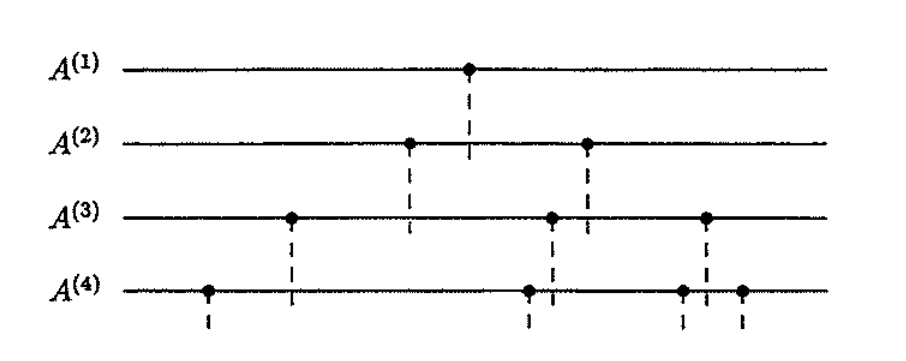
\includegraphics[width=0.8\textwidth]{Tekeningen/Interlacing.png}
  \centering
  \caption{Interlacing eigenschap (Trefethen en Bau, Figure 30.1)}
\end{figure}

Als voorbeeld wordt de volgende matrix gebruikt:\\

\[
A= 
\begin{bmatrix}
    1 & 1 & 0 & 0\\
    1 & 1 & -3 & 0\\
    0 & -3 & 1 & 2\\
    0 & 0 & 2 & 0
\end{bmatrix}
\]\\

De eigenwaarden van de submatrices zijn:\\

$k = 1: \lambda_{0}^{(1)} = 1$\\
$k = 2: \lambda_{0}^{(2)} = 0, \lambda_{1}^{(2)} = 2$\\
$k = 3: \lambda_{0}^{(3)} = -2.1623, \lambda_{1}^{(3)} = 1, \lambda_{2}^{(3)} = 4.1623$\\
$k = 4: \lambda_{0}^{(4)} = -2.8771, \lambda_{1}^{(4)} = 0, \lambda_{2}^{(4)} = 1.2874, \lambda_{3}^{(4)} = 4.5897$\\[10pt]

Voor deze matrix is de interlacing eigenschap dus bevestigd. Deze eigenschap kan dan in de volgende opgave gebruikt worden om de bisectiemethode toe te passen.\\

